%\documentclass[dvipdfmx,fleqn]{beamer}
\documentclass[dvipdfmx,fleqn,handout]{beamer}
\usepackage{amsmath,amssymb,amsthm}

\mode<presentation>
{
  \usetheme{default}
}

\title{\Large Fictitious play}
\author{\large 花嶋 陽}
\date{\small 6/28}

\usefonttheme{professionalfonts}

\setbeamercovered{transparent=20}

\setbeamertemplate{navigation symbols}{} 
\setbeamertemplate{footline}[frame number] 



\begin{document}

\sffamily
\gtfamily


\begin{frame}
  \titlepage
  \thispagestyle{empty}
\end{frame}

\setcounter{framenumber}{0}




\begin{frame}
\frametitle{はじめに}
\begin{itemize}\setlength{\parskip}{0.5em}
\item
Fictitious Playについて説明

\item
Matching Pennies ゲームを例にとった、
Fictitious Playのシュミレーションプログラムの
コードについて説明

\end{itemize}
\end{frame}



\begin{frame}
\frametitle{Ficititious playとは}
\begin{itemize}\setlength{\parskip}{0.5em}
\item
戦略形ゲームが$t=1,2,...$の各期にプレイされるとする。

\item
「$t+1$期に、他プレイヤーは1期からt期に選択した行動の比率に
等しい確率で各純戦略を選択する」と、各プレイヤーは予測する。 \pause


\item
各プレイヤーはその予測に対する最適反応戦略を選択する。 \pause

\item
このような動学モデルを"Fictitious Play"と言う。

\end{itemize}
\end{frame}

\begin{frame}
\frametitle{具体例 2×2ゲーム}
\begin{itemize}\setlength{\parskip}{0.5em}
\item
各期において0か1の行動をとる、プレイヤー0とプレイヤー1を用意する。

\item
t期において、プレイヤー0は
 \begin{itemize}\setlength{\parskip}{0.5em}
 \item
 プレイヤー1は確率$1-x_0(t)$で行動0をとる
 \item
 プレイヤー1は確率$x_0(t)$で行動1をとる
 \end{itemize}
と予測するとする。(プレイヤー1も同様)

\item
この下で、各プレイヤーは期待利得が最大になるように行動を決定する。(期待利得が等しい場合は等確率にどちらかを選ぶ)

\item
また、この$x_0(t)$ を
「t時点における、プレイヤー0の、プレイヤー1の行動に関する信念 (belief)」と呼ぶことにする。

\end{itemize}
\end{frame}

\begin{frame}
\frametitle{具体例 2×2ゲーム}
\begin{itemize}\setlength{\parskip}{0.5em}
\item
プレイヤー0の信念$x_0(t)$は次のように定まる。
 \begin{itemize}\setlength{\parskip}{0.5em}
 \item
 初期信念$x_0(0)$は[0,1]上の一様分布にしたがってランダムに与えられるとする。
 \item
 各$t\geq1$期において、プレイヤー1が過去とった行動を$a_1(0),...,a_1(t-1)$とすると、
 信念$x_0(t)$は、
 \[
 x_0(t)
 = \frac{x_0(0)+a_1(0)+...+a_1(t-1)}{t+1} 
 \]
 で与えられる。
 \item
 これは、
 \[
 x_0(t+1)
 = x_0(t) + \frac{1}{t+2} (a_1(t) - x_0(t))
 \]
 と再帰的に書くことができる。
 \end{itemize}
\end{itemize}
\end{frame}

\begin{frame}
\frametitle{具体例 2×2ゲーム}
\begin{itemize}\setlength{\parskip}{0.5em}
\item
つまりプレイヤー0とプレイヤー1を合わせて、
\[
x_0(t+1)
= x_0(t) + \frac{1}{t+2} (a_1(t) - x_0(t))
\]
\[
x_1(t+1)
= x_1(t) + \frac{1}{t+2} (a_0(t) - x_1(t))
\]
という連立1階漸化式を考えることになる。
\item
ただし、
 \begin{itemize}\setlength{\parskip}{0.5em}
 \item
 $a_0(t)$は$x_0(t)$に対する最適反応
 \item
 $a_1(t)$は$x_1(t)$に対する最適反応
 \item
 最適反応が複数あるときは等確率でランダムに選ぶ
 \end{itemize}
である。
\end{itemize}
\end{frame}

\begin{frame}[containsverbatim]
\frametitle{コードの説明}
\begin{itemize}\setlength{\parskip}{0.5em}
\item
Matching Pennies ゲームのシュミレーション
\item
Matching Pennies ゲームの利得表は以下の通り
\texttt{}
\[
\begin{pmatrix}
  1,-1&-1,1\\
  -1,1&1,-1
\end{pmatrix}
\]
\begin{verbatim}
ただし、行プレイヤーをプレイヤー0、列プレイヤーをプレイヤー1とし、
各プレイヤーの行動を行動0、行動1と呼ぶ。
\end{verbatim}
\end{itemize}
\end{frame}

\begin{frame}[containsverbatim]% verbatim 環境を使えるように
\frametitle{コードの説明}
\begin{itemize}\setlength{\parskip}{0.5em}
\item
コードの内容
\begin{verbatim}
# -*- coding: utf-8 -*-
from __future__ import division  
import matplotlib.pyplot as plt
from random import uniform, choice
import numpy as np

def fictplay(t):
    x_0_t = [uniform(0, 1)]
    x_1_t = [uniform(0, 1)]
#player0の利得
    gain_0 = np.array([[1, -1], [-1, 1]])
#player1の利得
     gain_1 = np.array([[-1, 1], [1, -1]]) 
	  
\end{verbatim}

\end{itemize}
\end{frame}

\begin{frame}[containsverbatim]% verbatim 環境を使えるように
\frametitle{コードの説明}
\begin{verbatim}
   for i in range(t):
   #probability: player1 choice 0 or 1
        pro_1 = np.array([1-x_0_t[i], x_0_t[i]])      
		   
   #expected gain = gain × probability          
      exp_gain_0 = np.dot(gain_0, pro_1)            
        
   #player0の最適反応
     if exp_gain_0[0] > exp_gain_0[1]:
            a_0_i = 0
        elif exp_gain_0[0] == exp_gain_0[1]:
            a_0_i = choice([0, 1])
        else:
            a_0_i = 1
                
                
\end{verbatim}

\end{frame}

\begin{frame}[containsverbatim]% verbatim 環境を使えるように
\frametitle{コードの説明}
\begin{verbatim}
        pro_0 = np.array([1-x_1_t[i], x_1_t[i]])   
        exp_gain_1 = np.dot(gain_1, pro_0)
		
    #player1の最適反応
        if exp_gain_1[0] > exp_gain_1[1]:
            a_1_i = 0
        elif exp_gain_1[0] == exp_gain_1[1]:
            a_1_i = choice([0, 1])
        else:
            a_1_i = 1
			   
    #i+1期の信念を計算
        x_0_i1 = x_0_t[i] + (a_1_i - x_0_t[i]) / (i+2)
        x_1_i1 = x_1_t[i] + (a_0_i - x_1_t[i]) / (i+2)
		      
        x_0_t.append(x_0_i1)
        x_1_t.append(x_1_i1)

    return x_0_t, x_1_t

\end{verbatim}

\end{frame}

\begin{frame}[containsverbatim]% verbatim 環境を使えるように
\frametitle{コードの説明}

\begin{verbatim}
x_0_t, x_1_t = fictplay(1000)
         
plt.plot(x_0_t, 'r-', label="x_0(t)")
plt.plot(x_1_t, 'b-', label="x_1(t)")
plt.legend()
#plt.savefig('matchingpennies_plot.pdf')
plt.show()

#x_0_t = []
#for i in range(100):
#    x_0, x_1 = fictplay(100)
#    x_0_t.append(x_0[-1])
#plt.hist(x_0_t, label="x_0(t)")
#plt.legend()
#plt.savefig('matchingpennies_plot1.pdf')
#plt.show()
\end{verbatim}
\end{frame}

\begin{frame}
\frametitle{図1}
\begin{figure}
 \centering
 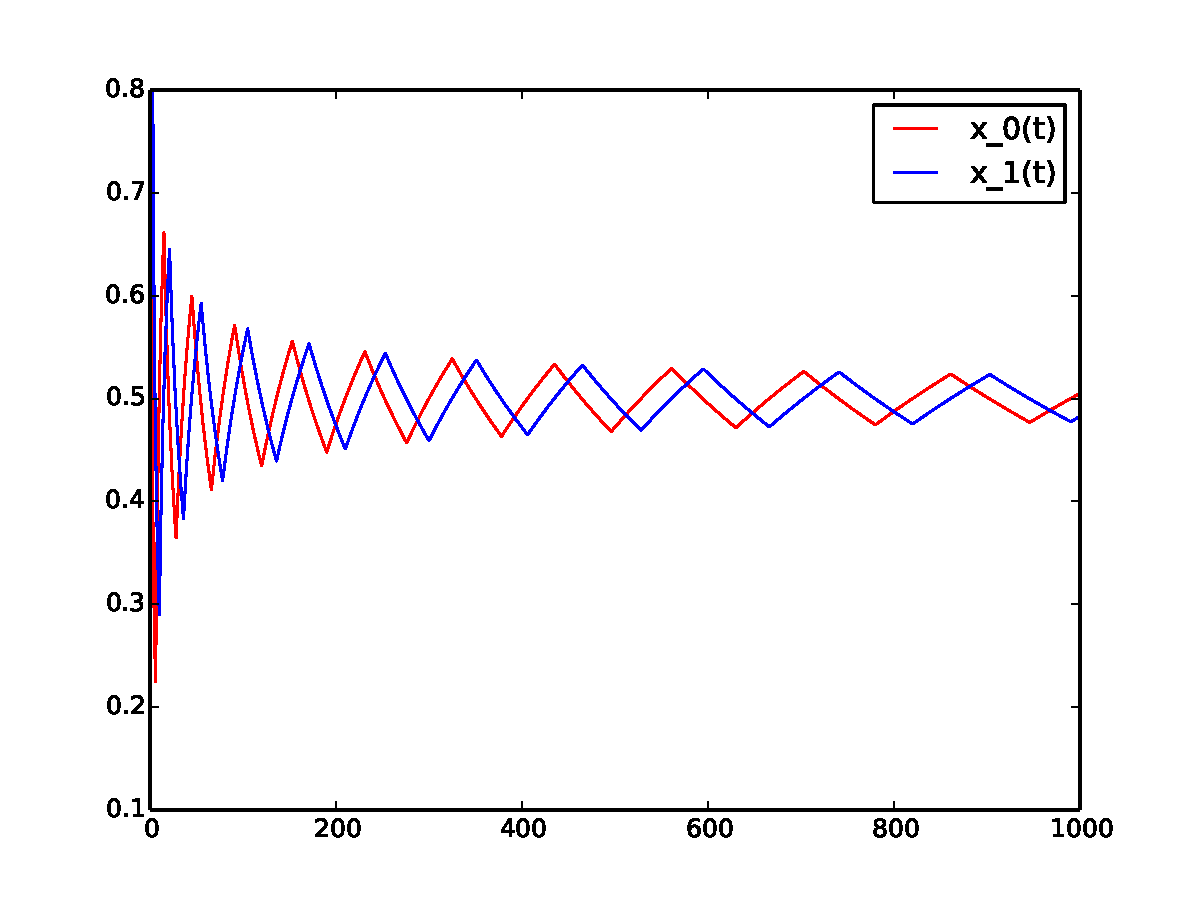
\includegraphics[scale=0.5]{matchingpennies_plot.pdf}
 \caption{t=1000期までの両プレイヤーの信念の推移}
 \label{fig:matchingpennies_plot}
\end{figure}
\end{frame}

\begin{frame}
\frametitle{図2}
\begin{figure}
 \centering
 \includegraphics[scale=0.5]{matchingpennies_plot1.pdf}
 \caption{100回シュミレーションした時の$x_0(t)$の値}
 \label{fig:matchingpennies_plot}
\end{figure}
\end{frame}


\begin{frame}
\frametitle{コードの説明 まとめ}
\begin{itemize}\setlength{\parskip}{0.5em}
\item
工夫した点
 \begin{itemize}\setlength{\parskip}{0.5em}
 \item
 期待利得を行列計算によって求めるようにした。
 \end{itemize}

\item
今後の課題
 \begin{itemize}\setlength{\parskip}{0.5em}
 \item
 プレイヤー0と1の最適反応を導くコードが重複しているので、うまく関数化したい。
 \end{itemize}
 
\end{itemize}
\end{frame}



\end{document}